\documentclass[11pt, a4paper]{article}

\usepackage{amsmath}
\usepackage{amssymb}
\usepackage{epsfig}
\usepackage{a4wide}
\usepackage{cancel}
\usepackage{subcaption}
\usepackage{appendix}

\graphicspath{{Figs/}}

\newcommand{\msp}{\mkern \medmuskip}

\newenvironment{braced}
 {\par\smallskip\hbox to\columnwidth\bgroup
  \hss$\left(\begin{minipage}{\columnwidth}}
 {\end{minipage}\right)$\hss\egroup\smallskip}


\title{\bf Introduction to Interferometry}
\author{Vasaant $^{\mbox{\tiny S}}$/$_{\mbox{\tiny O}}$ Krishnan\\
\texttt{kvasaant@ska.ac.za}}

\begin{document}

\maketitle

Radio interferometry is the technique of combining the response of multiple telescopes to detect radiation from astronomical sources. One of the main advantages of this technique is the resolution power of an interferometer. The angular resolution of any optical instrument can be approximated as~$\theta \sim \frac{\lambda}{D}$. So for any given wavelength of observation, $\lambda $, we obtain higher resolution by increasing the size of the aperture of the observing instrument,~$D$. However, this will eventually be limited by engineering constraints to~$\sim $100~metres for fully--steerable radio telescopes. With an interferometer,~$D$, is the separation \emph{between} the radio telescopes and can be as large as hundreds or even thousands of kilometres. In the following derivation, I will be providing a broad overview of the main concepts that interferometry is based upon.

\begin{figure}
  \centering
    \includegraphics[width=\textwidth ]{tms-figure.eps}
  \caption[]{A schematic diagram of interferometry showing the same electromagnetic plane wave~(the dotted line \textbf{-}\textbf{-}\textbf{-}\textbf{-}\textbf{-}\textbf{-}) from an astronomical source, in the direction,~$\mathbf{\hat{s}}$, incident upon antennas~$V_1$~and $V_2$. The angle~$\theta $ corresponds to the direction of~$\mathbf{\hat{s}}$ and gives rise to the different times at which this wave arrives at~$V_1$~and $V_2$. This time difference is given as~$\mathbf{\tau _g}$ corresponding to a distance of~$\mathbf{c\msp \tau_ g}$. The antennas $V_1$~and $V_2$ are separated along the baseline vector~$\vec{\mathbf{b}}$.\\ \emph{Image credit:} Interferometry and Synthesis in Radio Astronomy~(Thomson, Moran and Swenson,~2017) used under the Creative Commons Attribution International License (\texttt{http://creativecommons.org/licenses/by-nc/4.0/}). The bold, black lines and text have been added by me.}
  \label{fig:tms-figure}
\end{figure}

\section{Electromagnetic waves incident on an array}
The overall scheme of radio interferometry is represented in Figure~\ref{fig:tms-figure}. The incoming radiation from a natural astronomical source~\textbf{S} can be considered as a noise signal. Over a small time,~$\delta t$, the radiation can be considered to be sinusoidal. Such an oscillating electromagnetic wave with \emph{quasi--monochromatic} frequency,~$\nu $, can be described as

\begin{eqnarray}
  \label{eq:1}
  E(t) &=& A \msp cos(2\pi \msp \nu t + \Phi) \nonumber \\
       &=& A \msp cos(\omega t + \Phi) \msp , \hspace{0.8cm} \mbox{where} \enspace \omega = \frac{2\pi}{T} = 2\pi \nu
\end{eqnarray}

Our aim is to mathematically determine the relationship which will ensure that we are measuring the same wavefront of~$E(t)$ which is incident upon antennas~$V_1$ and~$V_2$. We do this by determining the \emph{geometric delay}~$\tau _g$, which is the time difference between the plane wave arriving at~$V_1$ and~$V_2$.

\begin{eqnarray}
  \label{eq:2}
  \tau _g &=& \frac{\mbox{Distance of the projection of $\vec{\mathbf{b}}$ in the direction of $\mathbf{\hat{s}}$}}{\mbox{Speed of light}} \nonumber \\
          &=& \frac{\vec{\mathbf{b}} \boldsymbol{\cdot} \mathbf{\hat{s}}}{c}
\end{eqnarray}

In Equation~\eqref{eq:2},~$\mathbf{\hat{s}}$ is a unit vector but~$\vec{\mathbf{b}}$ is not. This is because we do not know the distance to the source,~\textbf{S}. Having obtained an expression for~$\tau _g$, we can represent the electromagnetic radiation incident at the antennas as

\begin{eqnarray}
  \label{eq:3}
  \begin{aligned}
  V_1 &=& |V_1| \msp cos\big (\omega \msp (t - \tau _g)\big ) \\
  V_2 &=& |V_2| \msp cos(\omega t)
  \end{aligned}
\end{eqnarray}

\section{Correlation of a point source}
In signal processing \emph{cross--correlation} is the measure of similarity between two series which are offset from each other. In our system described in Equation~\eqref{eq:3} this offset is~$\omega \tau _g$.

We define the cross--correlation of the outputs of antennas~$V_1$ and~$V_2$ as~$<V_1V_2> = \frac{1}{T} \int _0^T V_1 \msp V_2 \msp dt$. It can be thought of as an \emph{averaging process} because you are integrating~(adding) over a certain duration and then dividing by the length of that duration.

% &=& \frac{1}{T} \int _0^T

\begin{eqnarray}
  \label{eq:4}
  <V_1V_2> &=& \frac{1}{T} \int _0^T V_1 \msp V_2 \msp d\,t \nonumber \\
           &=& \frac{1}{T}       \int _0^T |V_1| \msp cos(\omega \msp (t - \tau _g)) \enspace |V_2| \msp cos(\omega t) \msp d\,t \nonumber \\
           &=& \frac{1}{T} |V_1V_2| \int _0^T cos  \big (\omega \msp (t - \tau _g) + \omega t \big) + sin  \big (\omega \msp (t - \tau _g)\big) \msp sin(\omega t) \msp d\,t \nonumber \\
           &=& \frac{1}{T} |V_1V_2| \int _0^T cos(2\omega t - \omega \tau _g) - cos  \big (\omega (t - \tau _g) \big) \msp cos(\omega t) + cos  \big (\omega \msp (t - \tau _g) - \omega t \big) \msp d\,t \nonumber \\
           &=& \frac{1}{T} |V_1V_2| \int _0^T cos(2\omega t - \omega \tau _g) - cos  \big (\omega (t - \tau _g) \big) \msp cos(\omega t) + cos(-\omega \tau _g) \msp d\,t \nonumber \\
           &=& \frac{1}{T} |V_1V_2| \int _0^T cos(2\omega t - \omega \tau _g) - cos  \big (\omega (t - \tau _g) \big) \msp cos(\omega t) + cos(\omega \tau _g) \msp d\,t \nonumber \\
           &=& \frac{1}{T} |V_1V_2| \int _0^T cos(\omega \tau _g) + cos(2\omega t - \omega \tau _g) - cos  \big (\omega (t - \tau _g) \big) \msp cos(\omega t) \msp d\,t \nonumber \\
           &=& \frac{1}{T} |V_1V_2| \Bigg [ \int _0^T cos(\omega \tau _g) \msp dt + \int _0^T cos(2\omega t - \omega \tau _g) - cos  \big (\omega (t - \tau _g) \big) \msp cos(\omega t) \msp d\,t \Bigg ] \nonumber
\end{eqnarray}

In the last step, we have grouped the terms which depend on~$t$ in a single integral. In doing so we are attempting to make use of the following property: Over some sufficient duration of~$t \in \msp [\msp 0,~T\msp ]$, there will be sufficient complete cycles of the trigonometrical terms which depend on~$t$ for the result to average to~0 when integrating over~$d\,t$.\\

\begin{braced}
  Try integrating~$\int _0^{2\pi} sin(t) \msp dt $ or~$\int _0^{2\pi} cos(t) \msp dt $ to get an idea why this happens over complete trigonometric cycles.
\end{braced}

\begin{eqnarray}
  \label{eq:5}
  \implies \qquad <V_1V_2> &=& \frac{1}{T} |V_1V_2| \Bigg [\int _0^T cos(\omega \tau _g) \msp dt + 0 \Bigg ] \nonumber \\
           &=& \frac{1}{T} |V_1V_2| \enspace cos(\omega \tau _g) \msp \int _0^T 1 \msp dt \nonumber \\
           &=& \frac{1}{T} |V_1V_2| \enspace cos(\omega \tau _g) \msp \big[\msp t \msp \big]_0^T \nonumber \\
           &=& \frac{1}{T} |V_1V_2| \enspace cos(\omega \tau _g) \enspace T \nonumber \\
           &=& |V_1V_2| \enspace cos(\omega \tau _g)
\end{eqnarray}

In radio interferometry this process happens in the \emph{correlator}. The term~$|V_1V_2|$ is a multiplication of voltages which is proportional to power~(Ohm's Law: $P \propto V\mathcal{I} = V\frac{V}{R} = \frac{V^2}{R}$). I shall refer to~$|V_1V_2|$ as the intensity,~$I$, of the source which is the power per unit area.

\begin{eqnarray}
  \label{eq:6}
  \therefore \mbox{Correlator response,} \enspace R_c &=& <V_1V_2> \nonumber \\
                                                      &=& I \enspace cos(\omega \tau _g)
\end{eqnarray}

The correlator response,~$R_c$, is a function of~$\omega $ and~$\tau _g$. In practice~$\tau _g$ is difficult to time directly. So our aim now is to represent~$\tau _g$ in terms of quantities which we can measure easily, like:

\begin{enumerate}
  \itemsep-0.5cm
\item the baseline length~--~which \textbf{we} can measure from one antenna to another \\
\item the observation wavelength~--~dependant on the frequency range of the receivers \textbf{we} build \\
\item the position of the source in the sky~--~which is where \textbf{we} point the interferometer
\end{enumerate}

In expanding~$\tau _g$ in~$R_c$ we get

\begin{eqnarray}
  \label{eq:7}
  R_c &=& I \msp cos(\omega \tau _g) \nonumber \\
      &=& I \msp cos\Big (2\pi \msp \nu \msp \frac{\vec{\mathbf{b}} \boldsymbol{\cdot } \mathbf{\hat{s}}}{c}\Big ) \nonumber \\
      &=& I \msp cos\Big (2\pi \msp \nu \msp \frac{\vec{\mathbf{b}} \boldsymbol{\cdot } \mathbf{\hat{s}}}{\nu \msp \lambda}\Big ) \nonumber \\
      &=& I \msp cos\Bigg (2\pi \msp \frac{|b|\msp cos(\frac{\pi }{2} - \theta)}{\lambda}\Bigg ) , \hspace{0.8cm} \mbox{see Figure~\ref{fig:tms-figure}} \nonumber \\
      &=& I \msp cos\Big (2\pi \msp \frac{|b| \msp sin \theta}{\lambda} \Big) \nonumber \\
      &=& I \msp cos(2\pi \msp u \msp l) \msp , \hspace{0.8cm} \mbox{where} \enspace u = \frac{|b|}{\lambda}, \enspace l = sin \theta
\end{eqnarray}

Instead of using traditional units of distance, such as the meter, in interferometry it is more convenient to represent the baseline length in units of our observation frequency's corresponding wavelength, i.e.~$u = \frac{|b|}{\lambda}$.

\subsection{Visualising the correlator output}

We can graphically visualise the correlator output~$R_c$ by sketching the trigonometrical function~$R_c = I \msp cos(2\pi \msp u \msp l)$. The range of the cosine function~$R_c \in [-I, \msp I]$ for all values of~$u$ and~$l$. For this example let the baseline be~3~wavelengths long~$\implies u = \frac{|b|}{\lambda} = 3$ and our field--of--view extend from horizon--to--horizon~$\implies -\frac{\pi}{2} \leq \theta \leq \frac{\pi}{2}$.

\begin{eqnarray}
  \label{eq:8}
            \mbox{Maxima when} \qquad R_c &=& I           \nonumber \\
                  cos(2\pi \msp u \msp l) &=& 1           \nonumber \\
  \therefore \enspace 2\pi \msp u \msp l  &=& 2n \msp \pi \nonumber \\
       \frac{|b|}{\lambda} \msp sin\theta &=& n           \nonumber \\
                                   \theta &=& sin^{-1}\Big(\frac{n}{3}\Big) \msp , \hspace{0.8cm} \mbox{where} \enspace n \in \mathbb{Z}, \enspace |n| \leq 3 \nonumber \\
                                                 \nonumber \\
            \mbox{Minima when} \qquad R_c &=& -I \nonumber \\
                  cos(2\pi \msp u \msp l) &=& -1 \nonumber \\
   \therefore \enspace 2\pi \msp u \msp l &=& (2n+1) \msp \pi \nonumber \\
       \frac{|b|}{\lambda} \msp sin\theta &=& \frac{2n+1}{2} \nonumber \\
                                   \theta &=& sin^{-1}\Bigg(\frac{2n+1}{3 \msp (2)}\Bigg) \msp , \hspace{0.8cm} \mbox{where} \enspace n \in \mathbb{Z}, \enspace -3 \leq n < 3 \nonumber
\end{eqnarray}

\begin{table}
  \centering
\begin{tabular}{rrr}
  n & Maxima         & Minima         \\
  \hline
  $-$3 & $-$90.0$^\circ$ & $-$56.4$^\circ$ \\
  $-$2 & $-$41.8$^\circ$ & $-$30.0$^\circ$ \\
  $-$1 & $-$19.5$^\circ$ &  $-$9.6$^\circ$ \\
     0 &     0.0$^\circ$ &     9.6$^\circ$ \\
     1 &    19.5$^\circ$ &    30.0$^\circ$ \\
     2 &    41.8$^\circ$ &    56.4$^\circ$ \\
     3 &    90.0$^\circ$ &                \\
  \hline
\end{tabular}
\caption[]{Maxima and minima of~$R_c$ when~$u = \frac{|b|}{\lambda} = 3$.}
\label{tab:max-min}
\end{table}

%%BoundingBox: -30 210 600 684
\begin{figure}
  \centering
    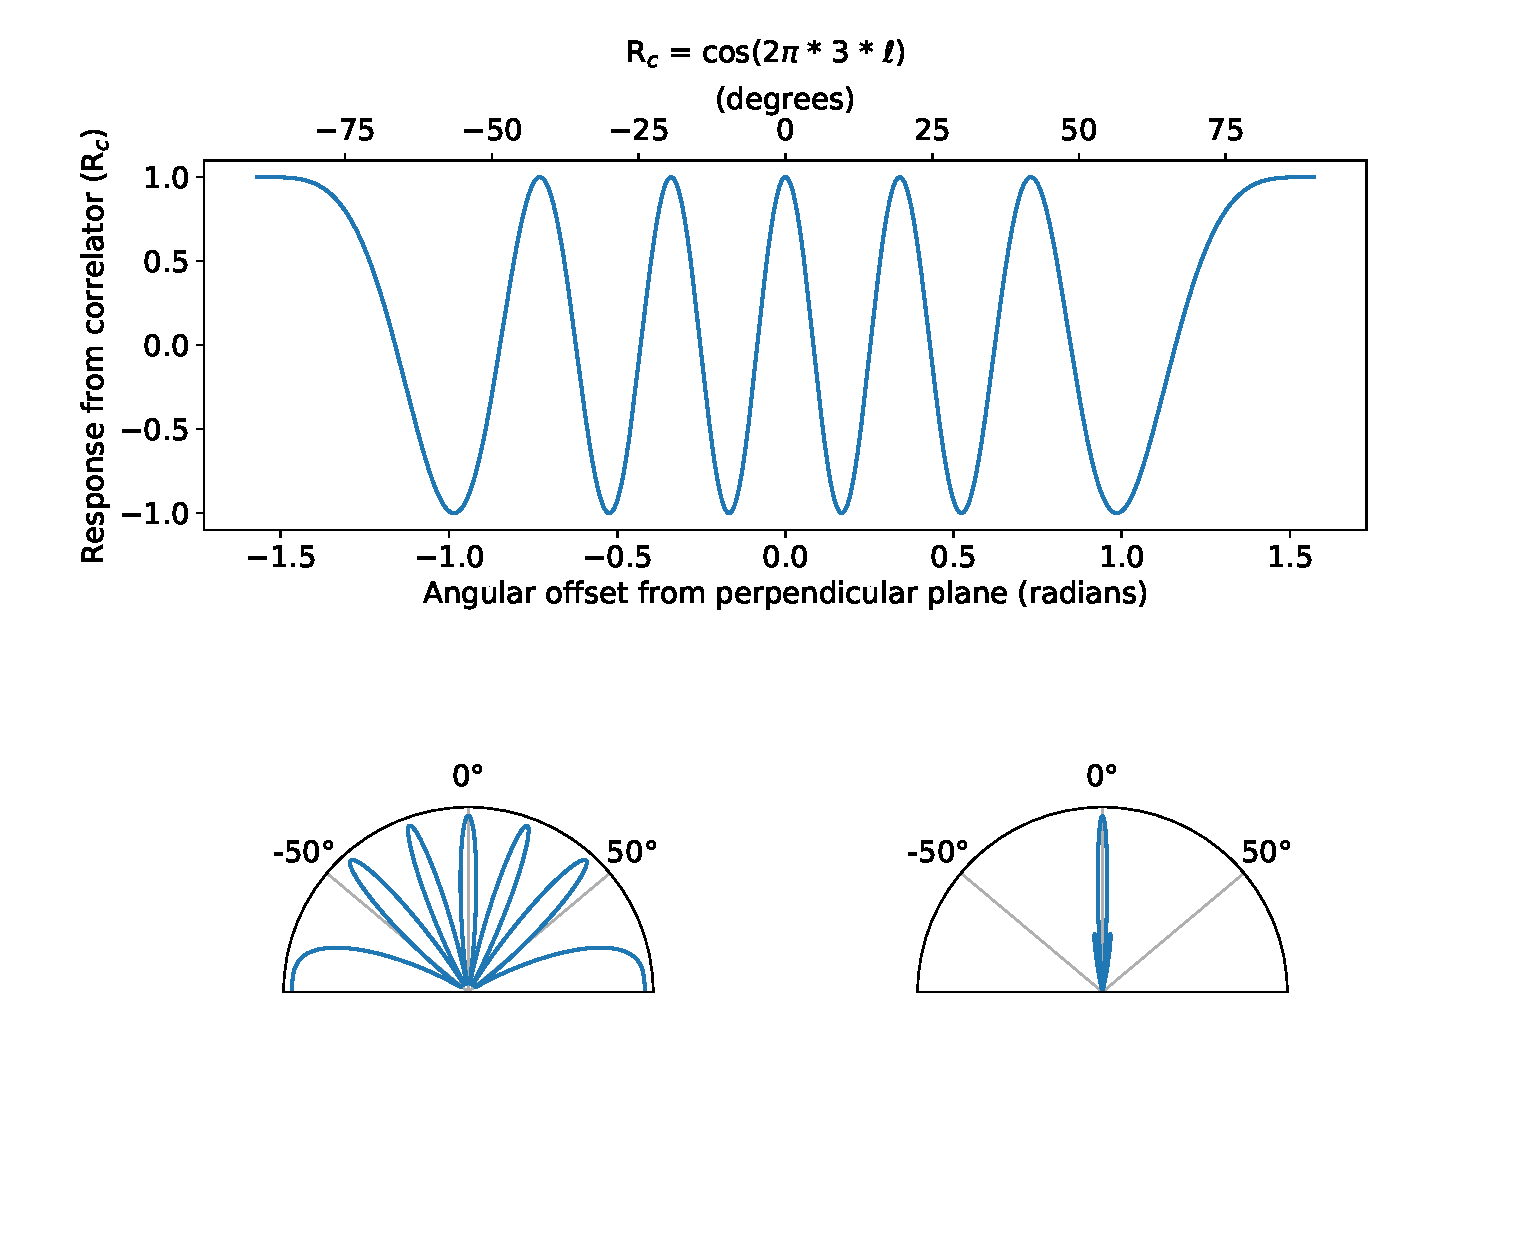
\includegraphics[width=\textwidth ]{01-corr-resp.eps}
  \caption[]{The correlator response,~$R_c$ in rectangular~(top) coordinates. The maxima and minima of~$R_c$ are stated in Table~\ref{tab:max-min}. The polar plot~(bottom left) shows what the fringes look like from horizon--to--horizon. The previous two plots resemble the response of a di--pole baseline. In contrast, the polar plot~(bottom right) resembles what you might expect from an interferometer like MeerKAT where there is a dominant central fringe and diminished sidelobes.}
  \label{fig:corr-resp}
\end{figure}

I show the maxima, minima of~$R_c$ in Table~\ref{tab:max-min}, and the corresponding curve in Figure~\ref{fig:corr-resp}. This curve is known as the interferometer's \emph{fringe pattern}, and you can think of it as the pattern which governs regions of the interferometer's sensitivity to the sky. In our example this would be the pattern for a dipole array. For interferometers such as MeerKAT, the fringes are shaped by the receivers such that the central lobe dominates. You can use \texttt{01-corr-resp.py} to determine the maxima, minima and fringe patterns for arbitrary values of~$u$ and~$l$.

At this point we can see why the interferometer's resolution power, which I described at the beginning as~$\theta \sim \frac{\lambda}{D}$ is what it is. We can do this by considering the separation of one maxima to the next in

\begin{eqnarray}
  \label{eq:10}
  \theta _{n+1} - \theta _n &=& sin^{-1}\Big(\frac{n+1}{u}\Big) - sin^{-1}\Big(\frac{n}{u}\Big) \nonumber \\
                           &\sim & \Big(\frac{n+1}{u}\Big) - \Big(\frac{n}{u}\Big) \msp , \hspace{0.8cm} \mbox{using the small angle approximation} \nonumber \\
                           &=& \frac{1}{u}       \nonumber \\
                           &=& \frac{\lambda}{b} \nonumber
\end{eqnarray}

% *** Also note that because |sin \theta| < 1, the number of lobes, %which is determined by n is < \frac{b}{\lambda}.

\section{Correlation of a non--point (finite) source}
\label{osec:Correlation-of-a-non-point-source}
Up to this point, we have considered the correlation of a point source. However, a real astronomical source occupies a~2\,D region on the \emph{celestial sphere}\footnote{The celestial sphere is an imaginary sphere which is concentric to Earth.}. For such an extended source we need to sum each of the antenna responses~--~$V_1$ and~$V_2$~--~~over a~2\,D solid angle region,~$d\,\Omega $, in the sky.

\begin{eqnarray}
  \label{eq:9}
  \therefore \enspace <V_1V_2> &=& \Big \langle \iint V_1 \msp d\,\Omega \iint V_2 \msp d\,\Omega \Big \rangle \nonumber
\end{eqnarray}

If \underline{and only if} the emission is \emph{spatially incoherent} then

\begin{eqnarray}
  \label{eq:19}
  \enspace <V_1V_2> &=& \Big \langle \iint V_1V_2 \msp d\,\Omega \Big \rangle \nonumber
\end{eqnarray}

\begin{braced}
  Spatial incoherence is required as in general~$\enspace \int g(x) \msp h(x) \msp d\,x \quad \neq \quad \int g(x) \msp d\,x \times \int h(x) \msp d\,x$.\\
  Typically we need to use \emph{integration by parts} in these cases.\\ For example try to integrate~$\quad \int x \msp cos(x) \msp d\,x \quad $ v.s.~$\quad \int x \msp d\,x \times \int cos(x) \msp d\,x$.
\end{braced}

\begin{eqnarray}
  \label{eq:11}
    &=& \frac{1}{T} \int _0 ^T \iint V_1 V_2 \msp d\,\Omega \enspace d\,t \nonumber \\
    &=& \iint \frac{1}{T} \int _0 ^T V_1 V_2 \msp d\,t \enspace d\,\Omega \nonumber \\
    &=& \iint I \msp cos(2\pi \msp u \msp l) \msp d\,\Omega
    % &=& \iint I_\nu (\hat{s}) \msp cos(2\pi \msp u \msp l) \msp d\,\Omega
    % &=& \iint I_\nu (\hat{s}) \msp e^{-i \msp 2\pi \msp \nu \msp \frac{\vec{b} \cdot \hat{s}}{c}} \msp d\,\Omega \nonumber
\end{eqnarray}

Note that the~$cos(2\pi \msp u \msp l)$ term in Equation~\eqref{eq:11} has a deficiency since the~$cos$ function is an \emph{even} function and is therefore only sensitive to the even component of the signal. We also need a way to detect/measure/sample the \emph{odd} component. This is because, for some general function

\begin{eqnarray}
  \label{eq:12}
  I(x) &=& I_{\mbox{\scriptsize even}}(x) + I_{\mbox{\scriptsize odd}}(x) \msp , \hspace{0.8cm} \mbox{for} -k \leq x \leq k \nonumber
\end{eqnarray}

The odd and even components have the property that

\begin{eqnarray}
  \label{eq:13}
  I_{\mbox{\scriptsize even}}(-x) &=& -I_{\mbox{\scriptsize even}}(x) \nonumber \\
  I_{\mbox{\scriptsize odd}}(-x)  &=&  I_{\mbox{\scriptsize odd}}(x) \nonumber \\
                                                              \nonumber \\
      \mbox{Giving} \qquad R_c &=& \iint I \msp cos(2\pi \msp u \msp l) \msp d\,\Omega \nonumber \\
                               &=& \iint \Big (I_{\mbox{\scriptsize even}} +  I_{\mbox{\scriptsize odd}} \Big ) \msp cos(2\pi \msp u \msp l) \msp d\,\Omega \nonumber \\
                               &=& \iint I_{\mbox{\scriptsize even}} \enspace cos(2\pi \msp u \msp l) + I_{\mbox{\scriptsize odd}} \enspace cos(2\pi \msp u \msp l) \msp d\,\Omega \nonumber \\
                               &=& \iint I_{\mbox{\scriptsize even}} \enspace cos(2\pi \msp u \msp l) \msp d\,\Omega + \iint I_{\mbox{\scriptsize odd}} \enspace cos(2\pi \msp u \msp l) \msp d\,\Omega \nonumber \\
                               &=& \iint I_{\mbox{\scriptsize even}} \enspace cos(2\pi \msp u \msp l) \msp d\,\Omega + \iint 0 \msp d\,\Omega \nonumber \\
                               &=& \iint I_{\mbox{\scriptsize even}} \enspace cos(2\pi \msp u \msp l) \msp d\,\Omega \nonumber
\end{eqnarray}

\begin{braced}
 To see why~$\iint I_{\mbox{\scriptsize even}} \enspace cos(2\pi \msp u \msp l) \msp d\,\Omega = 0$, try integrating $\int_{0}^{2\pi }cos(x)\msp cos(x) \msp d\,x$ v.s. $\int_{0}^{2\pi }sin(x)\msp cos(x) \msp d\,x$ or $\int_{-1}^{1}|x| \msp cos(x) \msp d\,x$ v.s. $\int_{-1}^{1} x \msp cos(x) \msp d\,x$.\\
\end{braced}

\subsection{Odd and Even Components of the Correlator Output}
So, if we wish to keep the odd component of the emission, we need to sample the~$sin$ component, which can be accomplished by generating a~90$^\circ $ phase shift in one of the signal paths from the pair of Equation~\eqref{eq:3}

\begin{eqnarray}
  \label{eq:14}
  \begin{aligned}
  V_1 &=& |V_1| \msp cos\big (\omega \msp (t - \tau _g)\big ) \\
  V_2 &=& |V_2| \msp cos\big (\omega t - \frac{\pi }{2}\big )
  \end{aligned}
\end{eqnarray}

In cross--correlating these antenna outputs~(as we did to obtain Equation~\eqref{eq:4})

\begin{eqnarray}
  \label{eq:15}
  <V_1V_2> &=& \frac{1}{T} \int _0^T V_1 \msp V_2 \msp dt \nonumber \\
           &=& \frac{1}{T}       \int _0^T |V_1| \msp cos(\omega \msp (t - \tau _g)) \enspace |V_2| \msp cos \big (\omega t - \frac{\pi }{2} \big ) \msp dt \nonumber \\
           &=& \frac{1}{T} |V_1V_2| \int _0^T cos  \big (\omega \msp (t - \tau _g) + \omega t - \frac{\pi }{2}\big) + sin \big (\omega \msp (t - \tau _g) \big) \msp sin(\omega t - \frac{\pi }{2} \big ) \msp dt \nonumber \\
           &=& \frac{1}{T} |V_1V_2| \int _0^T cos \big (2\omega t - \omega \tau _g - \frac{\pi }{2} \big ) - cos \big (\omega (t - \tau _g) \big) \msp cos \big (\omega t  -\frac{\pi }{2} \big ) + \dotso \nonumber \\
           && \dotso \enspace cos \Big [\omega \msp (t - \tau _g) - \big (\omega t - \frac{\pi }{2} \big ) \Big ] \msp dt \nonumber \\
           &=& \frac{1}{T} |V_1V_2| \int _0^T cos \big (2\omega t - \omega \tau _g - \frac{\pi }{2} \big ) - cos \big (\omega (t - \tau _g) \big) \msp cos \big (\omega t  -\frac{\pi }{2} \big ) + cos \big (\omega \tau _g - \frac{\pi }{2} \big ) \msp dt \nonumber \\
           &=& \frac{1}{T} |V_1V_2| \Bigg [\int _0^T cos \big (\omega \tau _g - \frac{\pi }{2} \big ) \msp dt + \dotso \nonumber \\
           && \dotso \enspace \int _0^T cos \big (2\omega t - \omega \tau _g - \frac{\pi }{2} \big ) - cos \big (\omega (t - \tau _g) \big) \msp cos \big (\omega t  -\frac{\pi }{2} \big ) \msp dt \Bigg ] \nonumber
\end{eqnarray}

Again we have the rapidly varying terms averaging to~0 and we substitute~$I$ for~$|V_1V_2|$.

\begin{eqnarray}
  \label{eq:16}
  \implies \qquad <V_1V_2> &=& \frac{1}{T} \msp I \Bigg [\int _0^T cos \big ( \omega \tau _g - \frac{\pi }{2}\big ) \msp dt + 0 \Bigg ] \nonumber \\
                           &=& I \msp cos \big ( \omega \tau _g - \frac{\pi }{2}\big )\nonumber \\
                           &=& I \msp \Big [cos(\omega \tau _g) \msp cos \big ( \frac{\pi }{2}\big ) + sin(\omega \tau _g) \msp sin \big ( \frac{\pi }{2}\big ) \Big ] \nonumber \\
                           &=& I \msp sin(\omega \tau _g) \nonumber \\
                                                          \nonumber \\
   \therefore \enspace R_s &=& I \msp sin(\omega \tau _g) \nonumber
\end{eqnarray}

The next natural step is to define a complex function in terms of the~$sin$ and~$cos$ components of the correlator output.

\begin{eqnarray}
  \label{eq:17}
  \therefore \enspace <V_1V_2> &=& R_c - i \msp R_s \msp , \hspace{0.8cm} \mbox{where} \enspace i = \sqrt{-1} \nonumber \\
                               &=& I \msp cos(\omega \tau _g) - i \msp I \msp sin(\omega \tau _g) \nonumber \\
                               &=& I \msp e^{-i\msp \omega \tau _g} \nonumber \\
                               &=& I \msp e^{-i\msp 2\pi \msp u \msp l}, \hspace{0.8cm} \mbox{see Equation~\eqref{eq:7} for converting } \omega \tau _g \mbox{ to } 2\pi \, u \, l \nonumber
\end{eqnarray}

\begin{braced}
  We use~$R_c - i \msp R_s$ instead of~$R_c + i \msp R_s$ to maintain the convention of the Fourier Transform relationship which will be revealed in Equation~\eqref{eq:24}.
\end{braced}
\vspace{0.5cm}

In conjunction with Equation~\eqref{eq:11} the correlator output is now called the \emph{complex visibility} and is given by

\begin{eqnarray}
  \label{eq:21}
  \begin{aligned}
  \mathcal{V}(\vec{b}) &=& \iint I_\nu (\hat{s}) \msp e^{-i \msp 2\pi \msp \nu \msp \frac{\vec{\mathbf{b}} \boldsymbol{\cdot} \mathbf{\hat{s}}}{c}} \msp d\,\Omega \\
                       &=& \iint I_\nu (\hat{s}) \msp e^{-i \msp 2\pi \msp \msp u \msp l} \msp d\,\Omega
  \end{aligned}
\end{eqnarray}

I have replaced~$I$ with,~$I_\nu (\hat{s})$ which is now the source brightness intensity at observing frequency~$\nu $ and in the direction~$\hat{s}$. At this stage, we are beginning to link something that we can measure, $\mathcal{V}(\vec{b}) = <V_1V_2>$, with something that we want to obtain,~$I_\nu (\hat{s})$.

% \begin{figure}
%   \centering
%   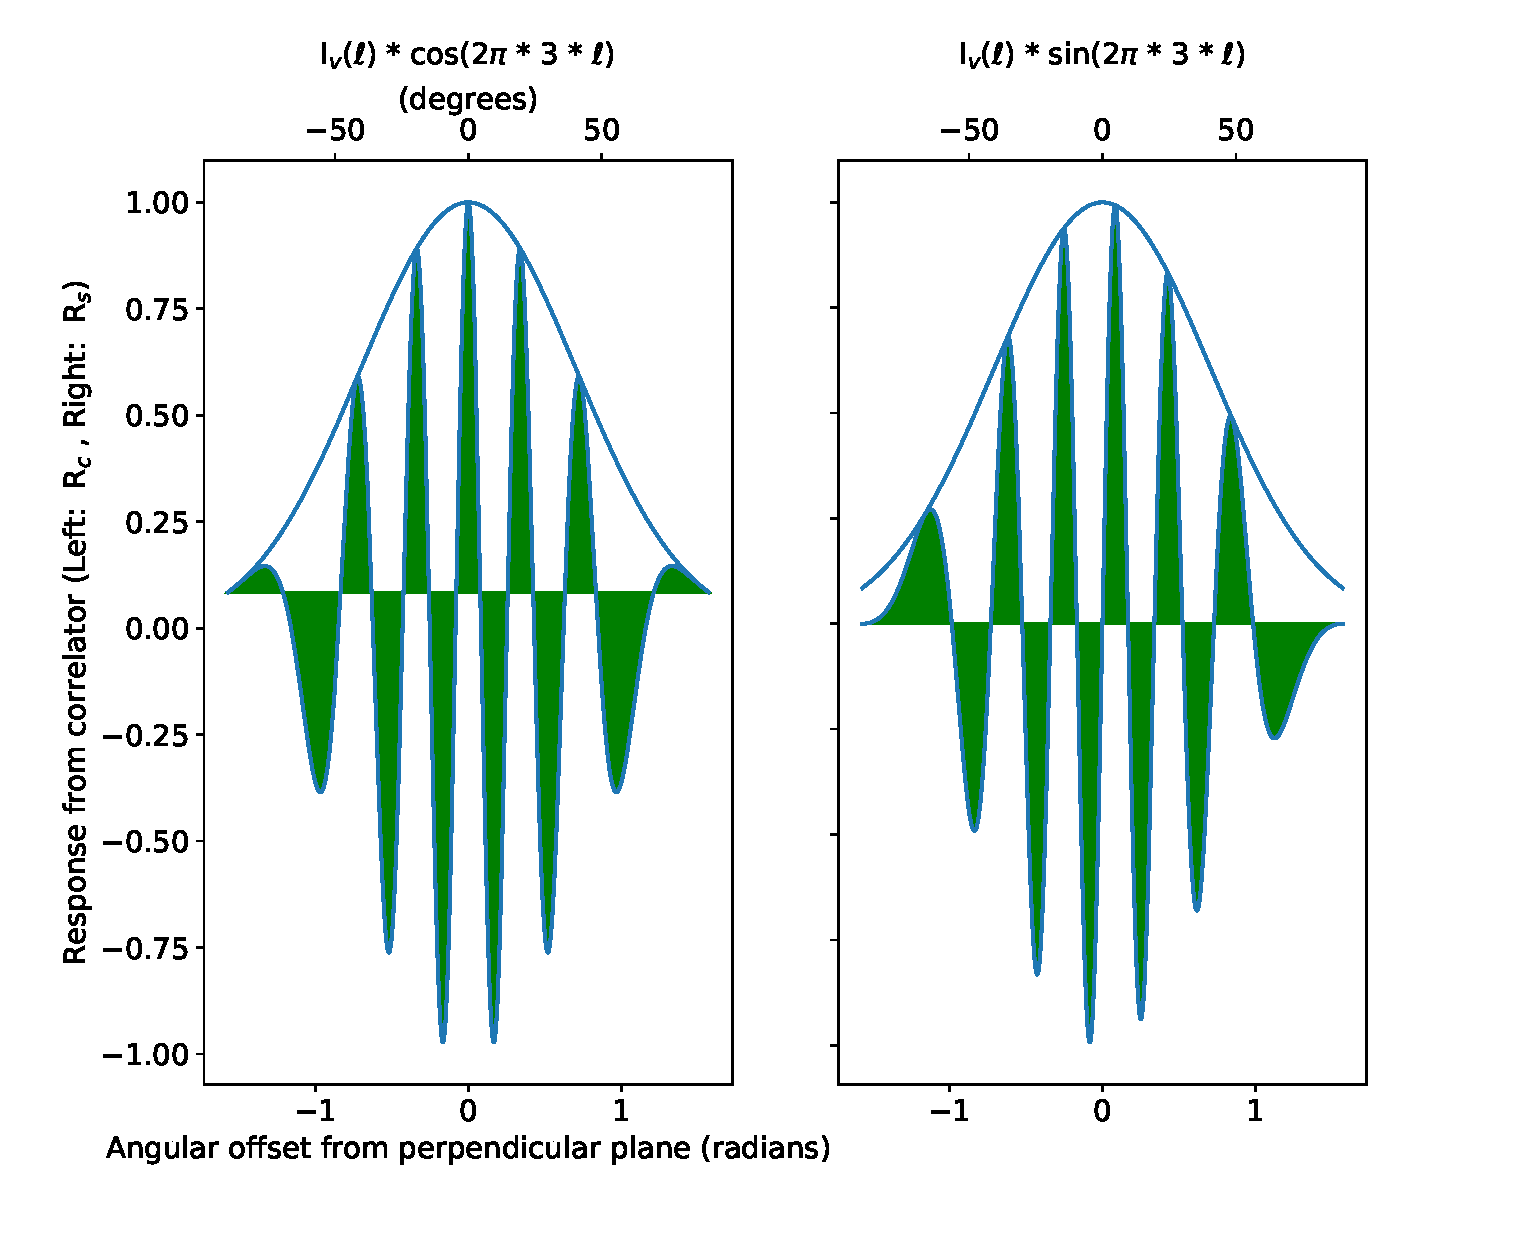
\includegraphics[width=\textwidth ]{02-vis-plot.eps}
%   \caption[]{The complex correlator response,~$\mathcal{V}$, showing both the~$cos$~(as in Figure~\ref{fig:corr-resp}) and~$sin$ components. Here the correlator is sampling a source with a \emph{Gaussian} power profile~$I = I_\nu (l) = e^{-l^2 }$ shown by the blue envelop.}
%   \label{fig:02-vis-plot}
% \end{figure}
% I give you an example of what the complex visibility might look like in Figure~\ref{fig:02-vis-plot}. Use~\texttt{02-vis-plot.py} to determine the fringe patterns for arbitrary values of~$u$ and~$l$.

\subsection{Visualising the result}
\label{sec:visualising-result}

Again, let's try to get an intuitive feel for what~$\mathcal{V}(\vec{b})$ is. In the following example, consider the simplest possible case where we have a~1\,D baseline such that~$\mathcal{V}(\vec{b}) = \mathcal{V}(u)$ which samples the source intensity along~1\,D such that~$I_\nu (\hat{s}) = I_\nu (l)$. $d\,\Omega $ now reduces to~$d\, l$. Furthermore, let us assume that the source intensity can be modelled as a~\emph{Dirac $\delta $--function} $\implies I_\nu (l) = \delta(l - l_0)$. $\mathcal{V}(\vec{b})$ can now be expressed as

\begin{eqnarray}
  \label{eq:25}
  \mathcal{V}(u) &=& \int \delta(l - l_0) \msp e^{-i \msp 2\pi \msp u \msp l} \msp d\,l \nonumber \\
                 &=& \int \delta(l - l_0) \msp e^{-i \msp 2\pi \msp u \msp l} \msp d\,l \Bigg \rvert_{\msp l \msp < \msp l_0} + \int \delta(l - l_0) \msp e^{-i \msp 2\pi \msp u \msp l} \msp d\,l \Bigg \rvert_{\msp l \msp = \msp l_0} + \int \delta(l - l_0) \msp e^{-i \msp 2\pi \msp u \msp l} \msp d\,l \Bigg \rvert_{\msp l \msp > \msp l_0} \nonumber \\
                                   &=& \int 0 \times e^{-i \msp 2\pi \msp u \msp l} \msp d\,l + \int \delta(0) \msp e^{-i \msp 2\pi \msp u \msp l_0} \msp d\,l + \int 0 \times e^{-i \msp 2\pi \msp u \msp l} \msp d\,l \nonumber \\
                                   &=& e^{-i \msp 2\pi \msp u \msp l_0} \msp \int \delta(0) \msp d\,l \nonumber \\
                                   &=& e^{-i \msp 2\pi \msp u \msp l_0} \msp \big [1\big ] \nonumber \\
                                   &=& cos(2\pi \msp u \msp l_0) - i \msp sin(2\pi \msp u \msp l_0) \nonumber
\end{eqnarray}

This means that the output of the correlator,~$\mathcal{V}(u)$, is just a complex number. In Figure~\ref{fig:03-dirac-vis}, we see~$\mathcal{V}(u)$ displayed in both trigonometrical form~(middle column) and amplitude \&~phase form~(right column), where the~$\mbox{amplitude} = \sqrt{cos^2 \msp (2\pi \msp u \msp l_0) - \msp sin^2 \msp (2\pi \msp u \msp l_0)} \msp = \msp 1$ and the~$\mbox{phase} = tan^{-1} \msp \Big [-\frac{sin(2\pi \msp u \msp l_0)}{cos(2\pi \msp u \msp l_0)} \Big ]$.

In Figure~\ref{fig:04-gauss-vis}, we add a level of complexity by replacing the~$I_\nu (l)$ in Equation~\eqref{eq:21} with a Gaussian function instead. Both these figures can be replicated using \texttt{03-dirac-vis.py} and \texttt{04-gauss-vis.py} for arbitrary source offsets, as well as source width for the latter case.

%% BoundingBox: 5 20 620 780 for fig = plt.figure(figsize=(10, 12))
\begin{figure}[]
  \centering
    \includegraphics[width=\textwidth ]{03-dirac-vis.eps}
  \caption{The output from the correlator,~$\mathcal{V}$ is always a complex number. Here we see~$\mathcal{V}$ in trigonometric~(middle column) and amplitude \&~phase~(right column) for the simplest case where~$\mathcal{V}(\vec{b}) = \mathcal{V}(u)$ and a source~$I_\nu (\hat{s}) = I_\nu (l) = \delta(l - l_0)$, which is offset from the phase centre by~$l \msp = \msp 0, \msp 2 \msp \mbox{\&} \msp 7$ units~(left column). The phase in the right column~$\in \msp [-\frac{\pi }{2}, \msp \frac{\pi }{2}]$~radians.}
  \label{fig:03-dirac-vis}
\end{figure}

%% BoundingBox: 5 20 620 780 for fig = plt.figure(figsize=(10, 12))
\begin{figure}
  \centering
    \includegraphics[width=\textwidth ]{04-gauss-vis.eps}
  \caption{The correlator response to different Gaussian functions.}
  \label{fig:04-gauss-vis}
\end{figure}

\section{Finite bandwidth}

The bandwidth has a dramatic effect on the correlator response. In the following computation, I am ignoring the effect of source structure.

\begin{eqnarray}
  \mathcal{V}(\vec{b}) &=& \iint I_\nu (\hat{s}) \msp e^{-i \msp 2\pi \msp \nu \msp \frac{\vec{\mathbf{b}} \boldsymbol{\cdot} \mathbf{\hat{s}}}{c}} \msp d\,\Omega \hspace{0.8cm} \longleftarrow \mbox{quasi--monochromatic, i.e. infinitesimal bandwidth} \nonumber \\
&=& \iint I_\nu (\hat{s}) \msp \frac{1}{\Delta \nu } \int ^{\nu_ 0 + \frac{\Delta \nu }{2}} _{\nu_ 0 + \frac{\Delta \nu }{2}} e^{-i \msp 2\pi \msp \nu \msp \frac{\vec{\mathbf{b}} \boldsymbol{\cdot} \mathbf{\hat{s}}}{c}} \msp d\, \nu \msp d\,\Omega \hspace{0.8cm} \longleftarrow \mbox{finite bandwidth} \nonumber \\
&=& \iint I_\nu (\hat{s}) \msp \frac{1}{\Delta \nu } \int ^{\nu_ 0 + \frac{\Delta \nu }{2}} _{\nu_ 0 + \frac{\Delta \nu }{2}} e^{-i \msp 2\pi \msp \nu \msp \tau _g} \msp d\, \nu \msp d\,\Omega \nonumber \\
&=& \iint I_\nu (\hat{s}) \msp \frac{1}{\Delta \nu } \int ^{\nu_ 0 + \frac{\Delta \nu }{2}} _{\nu_ 0 + \frac{\Delta \nu }{2}} cos(2\pi \msp \nu \msp \tau _g) - i \msp sin(2\pi \msp \nu \msp \tau _g)  \msp d\, \nu \msp d\,\Omega \nonumber \\
&=& \iint I_\nu (\hat{s}) \msp \frac{1}{\Delta \nu } \Bigg [\frac{sin(2\pi \msp \nu \msp \tau _g)}{2\pi \msp \tau _g} + i \msp \frac{cos(2\pi \msp \nu \msp \tau _g)}{2\pi \msp \tau _g}\Bigg ]^{\nu_ 0 + \frac{\Delta \nu }{2}} _{\nu_ 0 + \frac{\Delta \nu }{2}} \msp d\,\Omega \nonumber \\
&=& \iint I_\nu (\hat{s}) \msp \frac{1}{\Delta \nu \msp 2\pi \msp \tau _g} \Big [sin(2\pi \msp \nu \msp \tau _g) + i \msp cos(2\pi \msp \nu \msp \tau _g)\Big ]^{\nu_ 0 + \frac{\Delta \nu }{2}} _{\nu_ 0 + \frac{\Delta \nu }{2}} \msp d\,\Omega \nonumber \\
&=& \iint I_\nu (\hat{s}) \msp \frac{1}{2\pi \msp \tau _g \msp \Delta \nu} \Bigg [sin\Big [2\pi \msp \big (\nu_ 0 + \frac{\Delta \nu }{2}\big ) \msp \tau _g\Big ] + i \msp cos\Big [2\pi \msp \big (\nu_ 0 + \frac{\Delta \nu }{2}\big ) \msp \tau _g\Big ] \dotso \nonumber \\
&& \dotso \enspace - sin\Big [2\pi \msp \big(\nu_ 0 - \frac{\Delta \nu }{2}\big ) \msp \tau _g\Big ] - i \msp cos\Big [2\pi \msp \big (\nu_ 0 - \frac{\Delta \nu }{2}\big ) \msp \tau _g\Big ]\Bigg ] \msp d\,\Omega \nonumber \\
&=& \iint I_\nu (\hat{s}) \msp \frac{1}{2\pi \msp \tau _g \msp \Delta \nu} \Bigg [sin\Big (2\pi \msp \nu_ 0 \msp \tau _g + 2\pi \msp \frac{\Delta \nu }{2} \msp \tau _g\Big ) + i \msp cos\Big (2\pi \msp \nu_ 0 \tau _g + 2\pi \msp \frac{\Delta \nu }{2} \msp \tau _g\Big ) \dotso \nonumber \\
&& \dotso \enspace - sin\Big (2\pi \msp \nu_ 0 \msp \tau _g - 2\pi \msp \frac{\Delta \nu }{2} \msp \tau _g\Big ) - i \msp cos\Big (2\pi \msp \nu_ 0 \msp \tau _g - \frac{\Delta \nu }{2} \msp \tau _g\Big )\Bigg ] \msp d\,\Omega \nonumber \\
&=& \iint I_\nu (\hat{s}) \msp \frac{1}{2\pi \msp \tau _g \msp \Delta \nu} \Bigg [sin (2\pi \msp \nu_ 0 \msp \tau _g) \msp cos\Big (2\pi \msp \frac{\Delta \nu }{2} \msp \tau _g\Big ) + cos(2\pi \msp \nu_ 0 \msp \tau _g) \msp sin\Big (2\pi \msp \frac{\Delta \nu }{2} \msp \tau _g\Big ) \dotso \nonumber \\
&& \dotso + i \msp cos (2\pi \msp \nu_ 0 \msp \tau _g) \msp cos\Big (2\pi \msp \frac{\Delta \nu }{2} \msp \tau _g\Big ) - i \msp sin(2\pi \msp \nu_ 0 \msp \tau _g) \msp sin\Big (2\pi \msp \frac{\Delta \nu }{2} \msp \tau _g\Big ) \dotso \nonumber \\
&& \dotso - sin (2\pi \msp \nu_ 0 \msp \tau _g) \msp cos\Big (2\pi \msp \frac{\Delta \nu }{2} \msp \tau _g\Big ) + cos(2\pi \msp \nu_ 0 \msp \tau _g) \msp sin\Big (2\pi \msp \frac{\Delta \nu }{2} \msp \tau _g\Big ) \dotso \nonumber \\
&& \dotso - i \msp cos (2\pi \msp \nu_ 0 \msp \tau _g) \msp cos\Big (2\pi \msp \frac{\Delta \nu }{2} \msp \tau _g\Big ) - i \msp sin(2\pi \msp \nu_ 0 \msp \tau _g) \msp sin\Big (2\pi \msp \frac{\Delta \nu }{2} \msp \tau _g\Big )\Bigg ] \msp d\,\Omega \nonumber
\end{eqnarray}

\begin{eqnarray}
 \label{eq:27}
&=& \iint I_\nu (\hat{s}) \msp \frac{1}{2\pi \msp \tau _g \msp \Delta \nu} \Bigg [\cancel{sin (2\pi \msp \nu_ 0 \msp \tau _g) \msp cos\Big (2\pi \msp \frac{\Delta \nu }{2} \msp \tau _g\Big )} + cos(2\pi \msp \nu_ 0 \msp \tau _g) \msp sin\Big (2\pi \msp \frac{\Delta \nu }{2} \msp \tau _g\Big ) \dotso \nonumber \\
&& \dotso \cancel{+ i \msp cos (2\pi \msp \nu_ 0 \msp \tau _g) \msp cos\Big (2\pi \msp \frac{\Delta \nu }{2} \msp \tau _g\Big )} - i \msp sin(2\pi \msp \nu_ 0 \msp \tau _g) \msp sin\Big (2\pi \msp \frac{\Delta \nu }{2} \msp \tau _g\Big ) \dotso \nonumber \\
&& \dotso \cancel{- sin (2\pi \msp \nu_ 0 \msp \tau _g) \msp cos\Big (2\pi \msp \frac{\Delta \nu }{2} \msp \tau _g\Big )} + cos(2\pi \msp \nu_ 0 \msp \tau _g) \msp sin\Big (2\pi \msp \frac{\Delta \nu }{2} \msp \tau _g\Big ) \dotso \nonumber \\
&& \dotso \cancel{- i \msp cos (2\pi \msp \nu_ 0 \msp \tau _g) \msp cos\Big (2\pi \msp \frac{\Delta \nu }{2} \msp \tau _g\Big )} - i \msp sin(2\pi \msp \nu_ 0 \msp \tau _g) \msp sin\Big (2\pi \msp \frac{\Delta \nu }{2} \msp \tau _g\Big )\Bigg ] \msp d\,\Omega \nonumber \\
&=& \iint I_\nu (\hat{s}) \msp \frac{1}{2\pi \msp \tau _g \msp \Delta \nu} \Bigg [2 \msp cos(2\pi \msp \nu_ 0 \msp \tau _g) \msp sin\Big (2\pi \msp \frac{\Delta \nu }{2} \msp \tau _g\Big ) - 2 i \msp sin(2\pi \msp \nu_ 0 \msp \tau _g) \msp sin\Big (2\pi \msp \frac{\Delta \nu }{2} \msp \tau _g\Big ) \Bigg ] \msp d\,\Omega \nonumber \\
&=& \iint I_\nu (\hat{s}) \msp \frac{2 \msp sin\Big (2\pi \msp \frac{\Delta \nu }{2} \msp \tau _g\Big ) }{2\pi \msp \tau _g \msp \Delta \nu} \Big [cos(2\pi \msp \nu_ 0 \msp \tau _g) - i \msp sin(2\pi \msp \nu_ 0 \msp \tau _g) \Big ] \msp d\,\Omega \nonumber \\
&=& \iint I_\nu (\hat{s}) \msp \frac{sin (\pi \msp \Delta \nu \msp \tau _g)}{\pi \msp \tau _g \msp \Delta \nu} \Big [cos(2\pi \msp \nu_ 0 \msp \tau _g) - i \msp sin(2\pi \msp \nu_ 0 \msp \tau _g) \Big ] \msp d\,\Omega \nonumber \\
&=& \iint I_\nu (\hat{s}) \msp \frac{sin (\pi \msp \Delta \nu \msp \tau _g)}{\pi \msp \tau _g \msp \Delta \nu} \msp e^{-i \msp 2\pi \msp \nu _0 \msp \tau _g} \msp d\,\Omega
\end{eqnarray}

What this tells us is that the correlator response~$e^{-i \msp 2\pi \msp \nu _0 \msp \tau _g}$ is modulated by the normalised~$sinc$ function~$\frac{sin (\pi \msp \Delta \nu \msp \tau _g)}{\pi \msp \tau _g \msp \Delta \nu}$ as shown in Figure~\ref{fig:05-fin-band}. From Equation~\eqref{eq:27}, we clearly have nulls in the envelope~--~where the response falls to 0~--~when the numerator in~$\frac{sin (\pi \msp \Delta \nu \msp \tau _g)}{\pi \msp \tau _g \msp \Delta \nu}$ is~0.

\begin{figure}
  \centering
  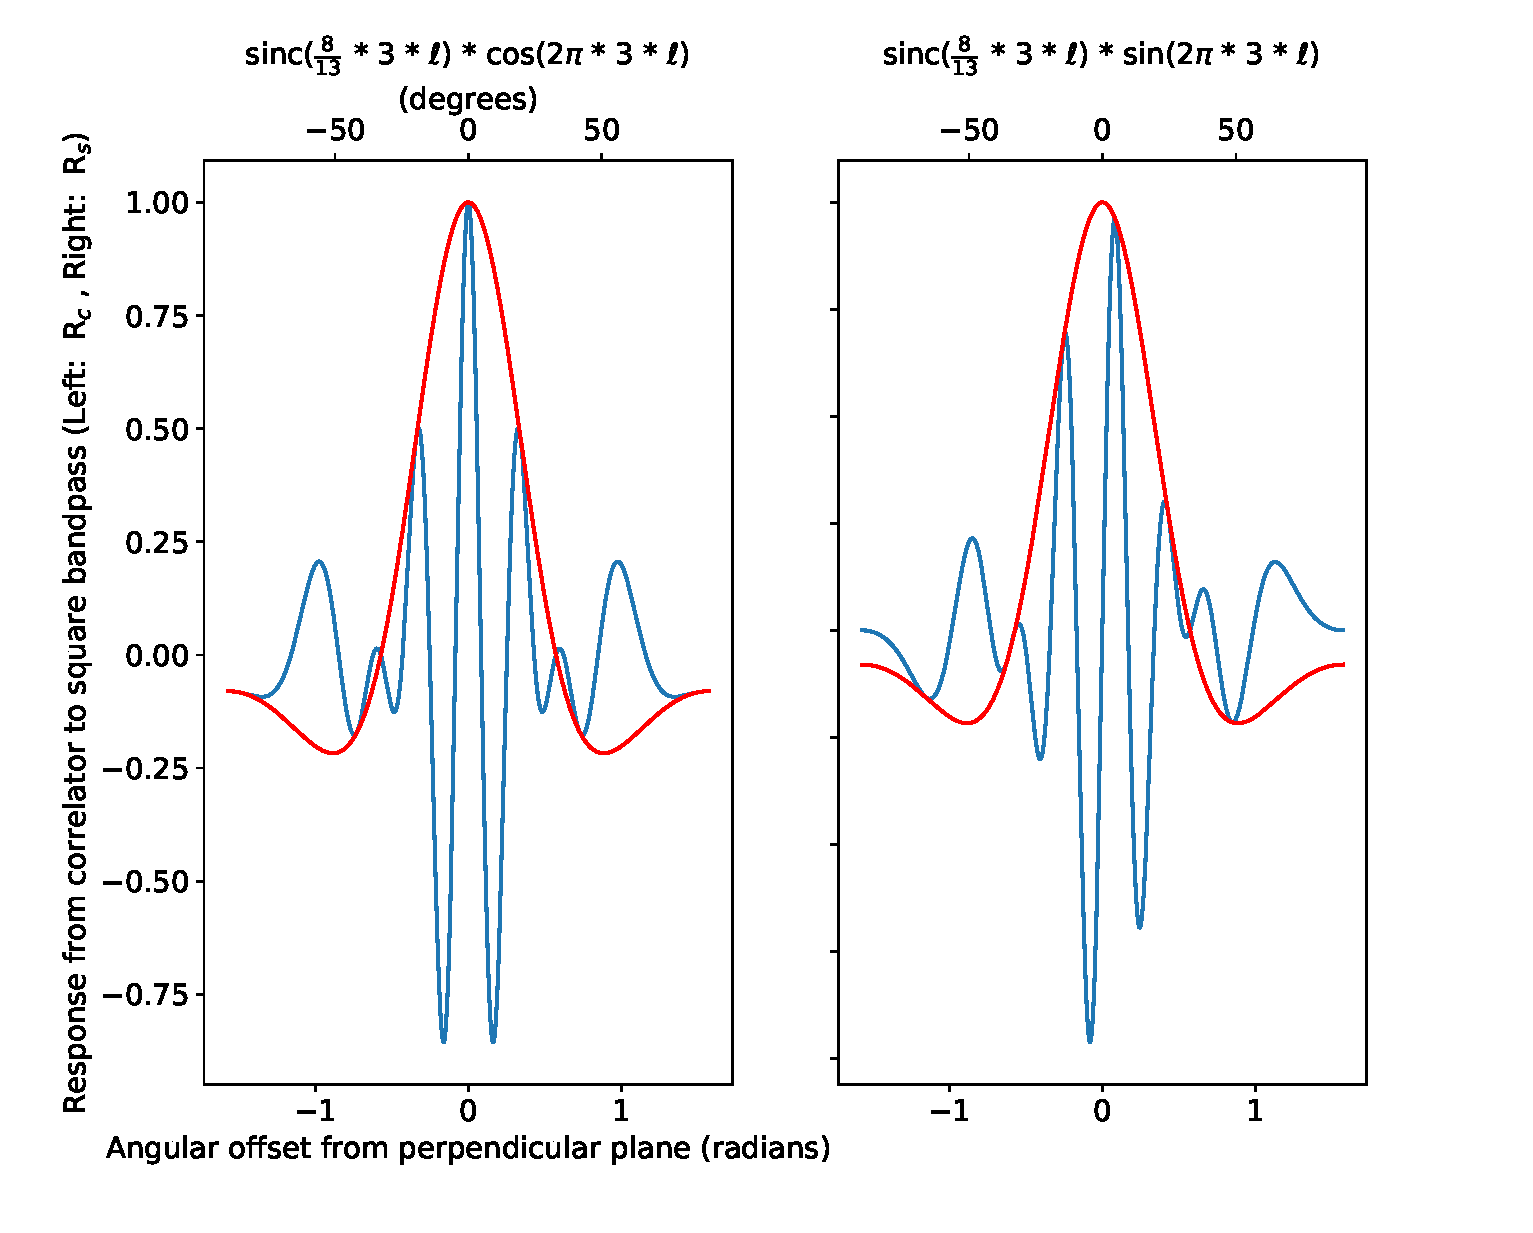
\includegraphics[width=\textwidth ]{05-fin-band-lecture.eps}
  \caption[]{The correlator~\emph{cosine}~(left) and~\emph{sine}~(right) responses (blue lines) when we have a finite--bandwidth of~$\Delta \nu = 8$~units~(e.g. GHz) and an observing frequency of~13~units for~$u = \frac{|b|}{\lambda} = 3$ and~$l$ extends from horizon--to--horizon~$\in [-\frac{\pi}{2},-\frac{\pi}{2}]$. The red line is the~\emph{sinc} envelope due to the bandwidth~$\Delta \nu $. This is analogous to Figure~\ref{fig:corr-resp}, except we assume an infinitesimal bandwidth and only a \emph{cosine} response in that previous figure. Use \texttt{05-fin-band.py} to replicate this figure.}
  \label{fig:05-fin-band}
\end{figure}

\begin{eqnarray}
  \label{eq:30}
  \mbox{i.e. when} \qquad sin (\pi \msp \Delta \nu \msp \tau _g) &=& 0 \nonumber \\
  \implies \qquad                       \Delta \nu \msp \tau _g  &=& 1 , \hspace{0.8cm} \mbox{for the first null}\nonumber \\
  \Delta \nu \msp  \frac{\vec{\mathbf{b}} \boldsymbol{\cdot} \mathbf{\hat{s}}}{c} &=& 1 \nonumber \\
  \Delta \nu \msp b \msp sin\theta &=& c \nonumber \\
  \therefore sin\theta &=& \frac{c}{b\msp \Delta \nu } \quad = \quad \frac{\frac{\lambda}{b}}{\frac{\Delta \nu }{\nu }} \nonumber
\end{eqnarray}

The number of fringes between the peak and this first null can be approximated by

\begin{eqnarray}
  \label{eq:31}
  N &\sim & \frac{\mbox{Distance between peak and first null}}{\mbox{Distance between fringes}} \nonumber \\
    &=&\frac{\frac{c}{b\msp \Delta \nu}}{\frac{\lambda }{b}} \nonumber \\
    &=& \frac{c}{b\msp \Delta \nu} \cdot \frac{b}{\lambda } \quad = \quad \frac{\nu }{\Delta \nu } \nonumber
\end{eqnarray}

i.e. something like observing frequency divided by the bandwidth. The~$sinc$ envelope can also be expressed in a way more useful to the interferometer's characteristics rather than~$\tau _g$ since~$sin(\pi \msp \tau _g \msp \Delta \nu ) = sinc \big (\pi \msp \frac{b}{\lambda } \msp \frac{\Delta \nu }{\nu } \msp sin\theta \big ) = sinc \big (\pi \msp \frac{b \msp \Delta \nu }{c} \msp sin\theta \big )$.

\section{Coordinate systems}

\begin{figure}
  \centering
    \includegraphics[angle= 90, width=0.75\textwidth ]{uv-lm-coords.eps}
    \caption[]{There are two coordinate frames which we use in interferometry. The source is in the~$l-m$ plane and the interferometer is in the~$u-v$ plane.\\ \emph{Image credit:} Interferometry and Synthesis in Radio Astronomy~(Thomson, Moran and Swenson,~2017) used under the Creative Commons Attribution International License (\texttt{http://creativecommons.org/licenses/by-nc/4.0/}). }
    \label{fig:uv-lm-coords}
\end{figure}

We need a formal coordinate framework in order to proceed further with the mathematics. This is described in Figure~\ref{fig:uv-lm-coords}. Let the baseline have components,~$\frac{\vec{b}}{\lambda } = u\,\hat{i} + v\,\hat{j} + w\,\hat{k}$. Let the source have components,~$\hat{s} = l\,\hat{i} + m\,\hat{j} + n\,\hat{k}$.

\begin{eqnarray}
  \label{eq:18}
\frac{\vec{\mathbf{b}}}{\lambda }\boldsymbol{\cdot} \mathbf{\hat{s}} = \frac{\vec{\mathbf{b}} \boldsymbol{\cdot} \mathbf{\hat{s}}}{\lambda } &=& (u\,\hat{i} + v\,\hat{j} + w\,\hat{k}) \cdot (l\,\hat{i} + m\,\hat{j} + n\,\hat{k}) \nonumber \\
                                         &=& (u\,l + v\,m + w\,n) \nonumber
\end{eqnarray}

\begin{braced}
Note that~$\hat{s}$ is a unit vector,~$|\hat{s}| = 1$.
\begin{eqnarray}
  \label{eq:20}
  \implies \qquad l^2 + m^2 + n^2 &=& 1 \nonumber \\
                                n &=& \sqrt{1 - l^2 + m^2} \nonumber
\end{eqnarray}
\end{braced}
\vspace{0.5cm}

At this point, we employ a simplification to assume that the antennas lie on a plane such that~$w = 0$.

\begin{eqnarray}
  \label{eq:22}
  \therefore \enspace \frac{\vec{\mathbf{b}} \boldsymbol{\cdot} \mathbf{\hat{s}}}{\lambda } &=& (u\,l + v\,m) \nonumber
\end{eqnarray}

Equation~\eqref{eq:21},~$\mathcal{V}(\vec{b}) = \iint I_\nu (\hat{s}) \msp e^{i \msp 2\pi \msp \nu \msp \frac{\vec{b} \cdot \hat{s}}{c}} \msp d\,\Omega $, now becomes

\begin{eqnarray}
  \label{eq:23}
  \mathcal{V}(\vec{b}) &=& \iint I_\nu (\hat{s}) \msp e^{-i \msp 2\pi \msp \nu \msp \frac{\vec{\mathbf{b}} \boldsymbol{\cdot} \mathbf{\hat{s}}}{c}} \msp d\,\Omega \nonumber \\
  \mathcal{V}(\vec{b}) &=& \iint I_\nu (\hat{s}) \msp e^{-i \msp 2\pi \msp \nu \msp \frac{\vec{\mathbf{b}} \boldsymbol{\cdot} \mathbf{\hat{s}}}{\nu \msp \lambda }} \msp d\,\Omega \nonumber \\
  \mathcal{V}(\vec{b}) &=& \iint I_\nu (\hat{s}) \msp e^{-i \msp 2\pi \msp \frac{\vec{\mathbf{b}} \boldsymbol{\cdot} \mathbf{\hat{s}}}{\lambda }} \msp d\,\Omega \nonumber \\
     \mathcal{V}(u, v) &=& \iint I_\nu (l, m) \msp e^{-i \msp 2\pi \msp (u\,l + v\,m)} \msp d\,l \msp d\,m \nonumber
\end{eqnarray}

In the final step, we replace the vectors~$\vec{\mathbf{b}}$ and~$\mathbf{\hat{s}}$ with their corresponding vector components~$u-v$ and~$l-m$. You can think of the area~$d\,\Omega \approx d\,l \msp d\,m$~(see the shaded area~$d\,\Omega $ in Figure~\ref{fig:uv-lm-coords}). We now have a~2\,D Fourier transform between the visibility,~$\mathcal{V}(u, v)$, which we can measure, and the source brightness distribution,~$I_\nu (l, m)$, which we want.

\begin{eqnarray}
  \label{eq:24}
  \begin{aligned}
  \mathcal{V}(u, v) &=& \iint I_\nu (l, m) \msp e^{-i \msp 2\pi \msp (u\,l + v\,m)} \msp d\,l \msp d\,m \\
  I_\nu (l, m) &=& \iint \mathcal{V}(u, v) \msp e^{ i \msp 2\pi \msp (u\,l + v\,m)} \msp d\,u \msp d\,v
  \end{aligned}
\end{eqnarray}

This is known as the \emph{Van Cittert--Zernicke Theorem} and~$I_\nu (l, m)$ is the \underline{\emph{true}} sky brightness distribution and~$\mathcal{V}(u, v)$ is the \underline{\emph{true}} sky visibility.

\section{UV sampling}

According to equation~\eqref{eq:24}, the source intensity~$I_\nu (l, m)$ can be perfectly described by~$\mathcal{V}(u, v)$. However, in practice this is not the case as the~$(u,\msp v)$ sampling is baseline dependent. Figure~\ref{fig:06-array2uv-triangle}~(left panel) shows a hypothetical triangular array with elements~$A$,~$B$ and~$C$. With respect to the centre~(0,\,0) of this array these have corresponding position vectors~$\overrightarrow{OA}$,~$\overrightarrow{OB}$ and~$\overrightarrow{OC}$. Since the~$u-v$ space is derived from the baseline vector, we need to determine the individual baseline coordinates~$\overrightarrow{AB}$,~$\overrightarrow{AC}$ and~$\overrightarrow{BC}$~(and corresponding degenerate baselines~$\overrightarrow{BA}$,~$\overrightarrow{CA}$ and~$\overrightarrow{CB}$). For example,

\begin{eqnarray}
  \label{eq:26}
  \overrightarrow{AB} &=&  \enspace \overrightarrow{AO} + \overrightarrow{OB} \nonumber \\
                      &=& -\overrightarrow{OA} + \overrightarrow{OB} \nonumber \\
                      &=& -(0.5\msp \hat{i} - 0.5\msp \hat{j}) + (0\msp \hat{i} + 0.5\msp \hat{j}) \nonumber \\
                      &=& -0.5\msp \hat{i} + 1\msp \hat{j} \nonumber
\end{eqnarray}

\begin{figure}
\begin{subfigure}[b]{\textwidth }
  \centering
  %%BoundingBox: -160 145 760 666 for fig = plt.figure(figsize=(15, 7.5))
  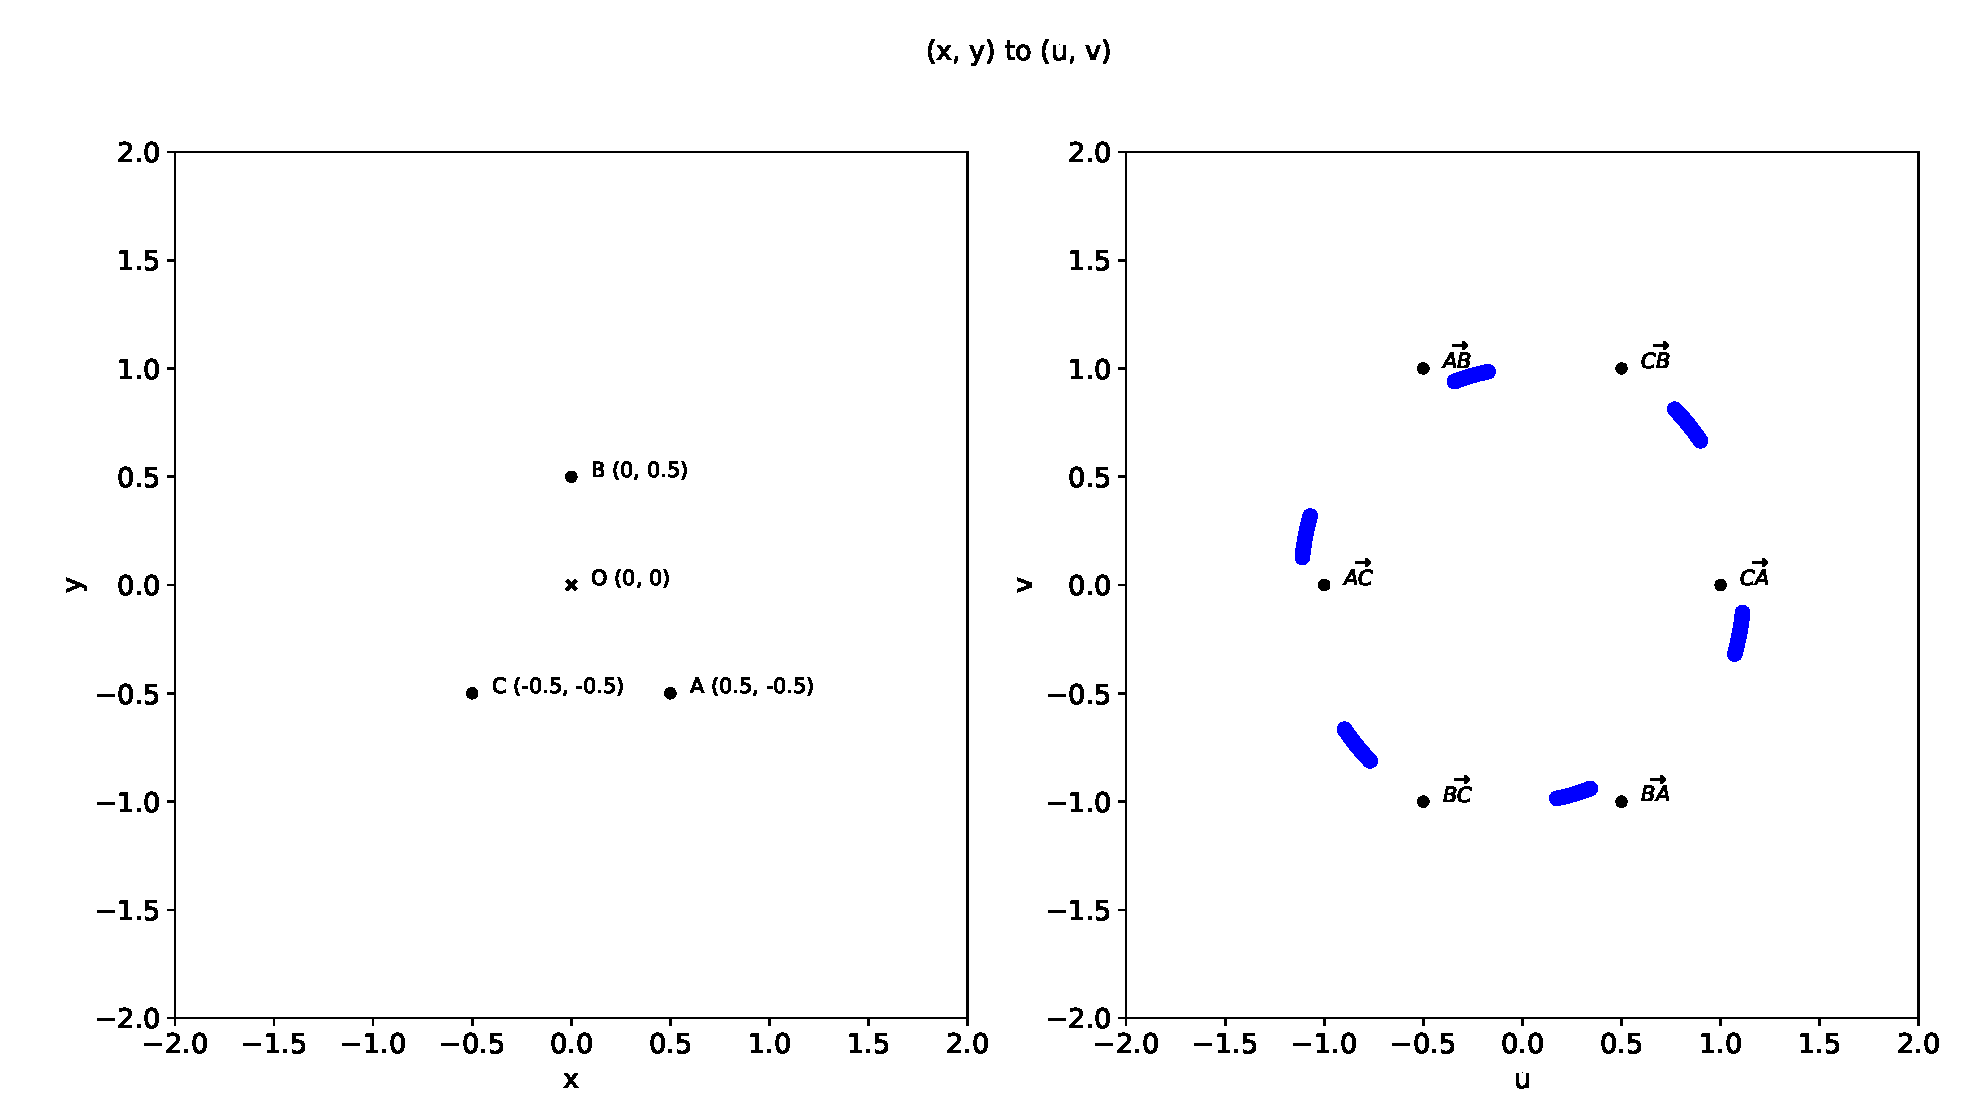
\includegraphics[width=\linewidth ]{06-array2uv-triangle.eps}
  \caption{The black circles represent antenna positions of a hypothetical array~(left panel) on the Earth's surface~($x,\msp y$) and corresponding~$uv$--coordinates~(right panel). The blue arcs trace the loci of these~$u-v$ points which are sampled as the Earth rotates. The offset between the start of the blue points and the black points is due to a coordinate rotation which I have applied in keeping with convention. You can use~\texttt{07-array2uv-loci.py} to reproduce this figure.\\}
  \label{fig:06-array2uv-triangle}
\end{subfigure}\\
\begin{subfigure}[b]{\textwidth }
  \centering
  %%BoundingBox: -175 145 760 666 for fig = plt.figure(figsize=(15, %7.5))
  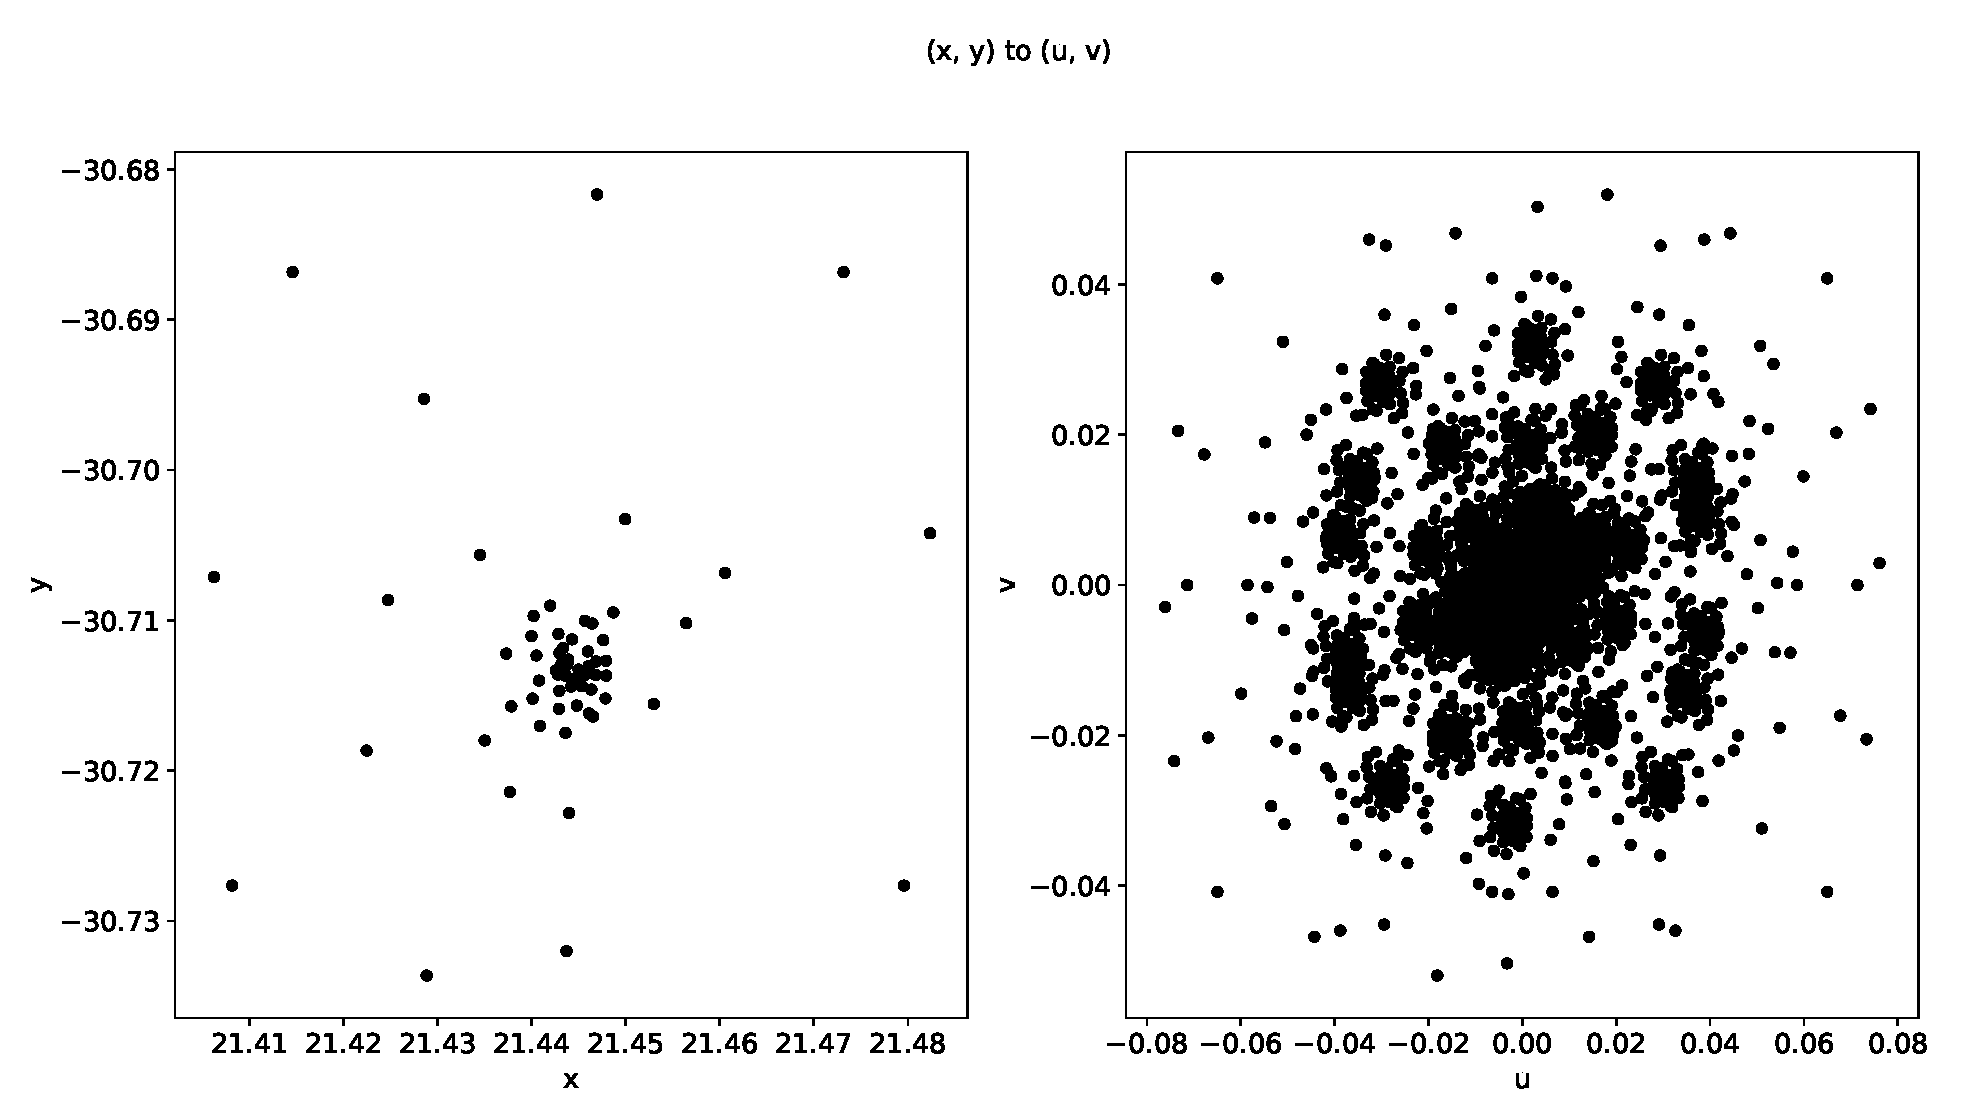
\includegraphics[width=\linewidth ]{06-array2uv-meerkat.eps}
  \caption{The black circles represent MeerKAT's antenna positions~(left panel) on the Earth's surface~($x,\msp y$) and corresponding~$uv$--coordinates~(right panel).}
  \label{fig:07-array2uv-meerkat}
\end{subfigure}
\caption{}
\label{fig:xy-uv}
\end{figure}

The right panel of Figure~\ref{fig:06-array2uv-triangle} is a graphical representation of what is known as the \emph{sampling pattern},~$S(u, v)$, because it is where~$\mathcal{V}(u, v)$ is sampled such that we have the \emph{dirty image}

\begin{eqnarray}
  \label{eq:28}
   \mbox{True image,} \quad I_\nu (l, m) &=& \iint \mathcal{V}(u, v) \msp e^{ i \msp 2\pi \msp (u\,l + v\,m)} \msp d\,u \msp d\,v \hspace{0.5cm} \mbox{from Equation~\eqref{eq:24}} \nonumber \\
   \mbox{Dirty image,} \quad I_{\mbox{\tiny{\emph{D}}}} (l, m) &=& \iint S(u, v) \msp \mathcal{V}(u, v) \msp e^{ i \msp 2\pi \msp (u\,l + v\,m)} \msp d\,u \msp d\,v
\end{eqnarray}

We know that a product of two functions in the~$u-v$ Fourier domain corresponds to a convolution of two signals in the~$l-m$ domain such that~$I_{\mbox{\tiny{\emph{D}}}} (l, m) = I_\nu (l,m) * B(l,m)$, where~$B(l,m)$ is known as the \emph{dirty beam} and is the Fourier Transform of~$S(u, v)$

\begin{eqnarray}
  \label{eq:29}
  B(l,m) &=& \iint S(u, v) \msp e^{ i \msp 2\pi \msp (u\,l + v\,m)} \msp d\,u \msp d\,v \nonumber
\end{eqnarray}

I have summarised the relationship between~$I_\nu (l, m)$, $\mathcal{V}(u,  v)$, $B(l, m)$, $S(u, v)$, $I_{\mbox{\tiny{\emph{D}}}}(l, m)$ and~$\mathcal{V}(u,  v) \msp S(u, v)$ in Table~\ref{tab:uv-summary}. Recovering~$I_\nu (l, m)$, $\mathcal{V}(u,  v)$ from~$I_{\mbox{\tiny{\emph{D}}}}(l, m)$ is a deconvolution problem which can be accomplished using~CLEAN.

\begin{table}
  \centering
  \begin{tabular}{r|ccccc}
$\mathbf{l-m}$ \textbf{(image)}     & $I_\nu (l, m)$            & * & $B(l, m)$               & = & $I_{\mbox{\tiny{\emph{D}}}}(l, m)$ \\
\textbf{domain}                     & True image               & & Dirty beam              &   & Dirty image                       \\
                                    & \emph{\textbf{(Desired)}}& & & & \\
                                    &                          & & & & \\
              $\mathcal{F.T.}$      & $\Big \Updownarrow $     & & $\Big \Updownarrow $    &   & $\Big \Updownarrow $              \\
                                    &                          & & & & \\
$\mathbf{u-v}$ \textbf{(Fourier)}   & $\mathcal{V}(u,  v)$     & $\times $ & $S(u, v)$               & = & $\mathcal{V}(u,  v) \msp S(u, v)$ \\
      \textbf{domain}               & True visibility          & & Sampling pattern        &   & \emph{\textbf{(Measured)}}        \\
                                    &                          & & \emph{\textbf{(Known)}} &   &                                   \\
  \end{tabular}
  \caption[]{A summary of the relationship between quantities in the image and Fourier domains.}
  \label{tab:uv-summary}
\end{table}

\section{Calibration}
\label{sec:calibration}
% Based on Chapter 10 of TMS.

The input visibilities are contaminated\footnote{e.g. antenna electronics, imperfect atmosphere over individual antennas, etc} by the time dependant complex \emph{baseline gains}~$\mathcal{G}_{ij}(t)$ for antennas~$i,\msp j$. The Fourier Transform of Equation~\eqref{eq:28} including~$\mathcal{G}_{ij}(t)$ is:
\begin{eqnarray}
  \label{eq:32}
  \big [\mathcal{V}(u,  v) \msp S(u, v)\big ]_{\mbox{\tiny uncal}} &=& \enspace \mathcal{G}_{ij}(t) \msp \iint I_{\mbox{\tiny D}} (l, m) \msp e^{-i \msp 2\pi \msp (u\,l + v\,m)} \msp d\,l \msp d\,m \nonumber \\
\end{eqnarray}

This means that the sampled target visibilities are

\begin{eqnarray}
  \label{eq:34}
\mathcal{V}(u,  v) \msp S(u, v) \quad = \quad \frac{\big [\mathcal{V}(u,  v) \msp S(u, v)\big ]_{\mbox{\tiny uncal}}}{\mathcal{G}_{ij}(t)} &=& \iint I_{\mbox{\tiny D}} (l, m) \msp e^{-i \msp 2\pi \msp (u\,l + v\,m)} \msp d\,l \msp d\,m
\end{eqnarray}

So we need to determine~$\mathcal{G}_{ij}(t)$ before we can obtain~$I_{\mbox{\tiny D}}$. The gain $\mathcal{G}_{ij}(t)$ for some baseline~$i,\msp j$ can be derived from regular observations of a calibrator source with visibilities~$\mathcal{V}_{\mbox{\tiny C}}(u, v)$. Such sources are

\begin{itemize}
\item[-] relatively strong (for signal--to--noise considerations)
\item[-] have a point--like structure
\item[-] have well--constrained astrometric\footnote{Astrometry is the science of measuring the positions of astronomical objects in the sky.} positions
\end{itemize}

If these three conditions are met~~(usually the case), then we have a situation which mimics the top row of panels in Figures~\ref{fig:03-dirac-vis} and~\ref{fig:04-gauss-vis}. Then the amplitude and the phase of the baseline~$i,\msp j$ are unequivocally known. If these conditions are all met, we force the measured calibrator visibilities~$\mathcal{V}_{\mbox{\tiny C}}(u, v)$ to be
\begin{eqnarray}
  \label{eq:33}
   \mathcal{V}_{\mbox{\tiny C}}(u, v) &=& \mathcal{G}_{ij}(t)\msp S_c \hspace{0.8cm} \mbox{for a calibrator with flux density }S_c \nonumber \\ \nonumber \\
  \therefore \quad \mbox{The baseline gains are} \quad \mathcal{G}_{ij}(t) &=& \frac{\mathcal{V}_{\mbox{\tiny C}}(u, v)}{S_{ij}} \nonumber \\ \nonumber \\
  \mbox{Hence Equation~\eqref{eq:34}} \quad \mathcal{V}(u,  v) \msp S(u, v) &=& \frac{\big [\mathcal{V}(u,  v) \msp S(u, v)\big ]_{\mbox{\tiny uncal}}}{\mathcal{G}_{ij}(t)} \hspace{0.8cm} \mbox{becomes} \nonumber \\ \nonumber \\
  \mathcal{V}(u,  v) \msp S(u, v) \enspace = \enspace \frac{\big [\mathcal{V}(u,  v) \msp S(u, v)\big ]_{\mbox{\tiny uncal}}}{\frac{\mathcal{V}_{\mbox{\tiny C}}(u, v)}{S_{ij}}} &=& \iint I_{\mbox{\tiny D}} (l, m) \msp e^{-i \msp 2\pi \msp (u\,l + v\,m)} \msp d\,l \msp d\,m \nonumber
\end{eqnarray}

\subsection{What do we do with~$\mathcal{G}_{ij}(t) = \frac{\mathcal{V}_{\mbox{\tiny C}}(u, v)}{S_{ij}}\msp $?}
Any wrapping in phase slopes~--~as seen in third columns of Figures~\ref{fig:03-dirac-vis} and~\ref{fig:04-gauss-vis} for the cases where there is a source offset~--~indicates that there is an error with the calibrator's astrometric position or due to baseline contaminants~--~or both. In Section~\ref{sec:calibration} we assume that the calibrator has a~``well--constrained astrometric position'' so any non--zero phase in~$\mathcal{V}_{\mbox{\tiny C}}(u, v)$ in Equation~\eqref{eq:33} is due to contaminants from~$\mathcal{G}_{ij}(t)$. So phase wrap is purely the instrumental phase and we subtract it from the observed phase.

\appendix
\appendixpage
\addappheadtotoc

\section{Velocity resolution}

\begin{eqnarray}
  \label{eq:39}
 \nu &=& \mbox{the observed frequency} \nonumber \\
 \nu_0 &=& \mbox{the observed frequency} \nonumber \\
 c &=& \mbox{the propagation speed of waves in the medium} \nonumber \\
 v_r &=& \mbox{the speed of the receiver relative to the medium} \nonumber \\
 v_s &=& \mbox{the speed of the source relative to the medium} \nonumber
\end{eqnarray}

The Doppler equation is given as

\begin{eqnarray}
  \label{eq:35}
  \nu &=& \Big (\frac{c + v _r}{c + v _s} \Big ) \msp \nu_0 \nonumber \\
  \nu &=& \Bigg (\frac{1 + \frac{v _r}{c}}{1 + \frac{v _s}{c}} \Bigg ) \msp \nu_0 \nonumber
\end{eqnarray}

For~$\frac{v _s}{c} \ll 1$ the denominator~$\frac{1}{1+\frac{v _s}{c}} \approx 1 - \frac{v _s}{c}$.

\begin{eqnarray}
  \label{eq:36}
  \implies \qquad \nu &=& \Big (1 + \frac{v _r}{c} \Big ) \Big (1 - \frac{v _s}{c} \Big ) \msp \nu_0 \nonumber \\
  \nu &=& \Big (1 + \frac{v _r - v _s}{c} - \frac{v _r\msp v _s}{c} \Big ) \msp \nu_0 \nonumber
\end{eqnarray}

Here $\frac{v _r\msp v _s}{c} \approx 0$, since~$\frac{v _s}{c} \ll 1$ and~$\frac{v _r}{c} \ll 1$

\begin{eqnarray}
  \label{eq:37}
  \implies \qquad\nu &=& \Big (1 + \frac{v _r - v _s}{c} \Big ) \msp\nu_0 \nonumber \\
 \nu &=&\nu_0 + \Big (\frac{v _r - v _s}{c} \Big ) \msp\nu_0 \nonumber \\
 \nu -\nu_0 &=& \frac{v _r - v _s}{c} \msp\nu_0 \nonumber
\end{eqnarray}

Giving the approximate Doppler Equation

\begin{eqnarray}
  \label{eq:38}
  \Delta \nu &=& \frac{\Delta v}{c} \msp \nu_0
\end{eqnarray}

So the velocity resolution is

\begin{eqnarray}
  \label{eq:41}
  \Delta v = \msp \frac{c \msp \Delta \nu }{\nu_0}
\end{eqnarray}

under the condition that~$\Delta \nu \ll \nu _0$.

\section{Converting source velocity to sky frequency}

\begin{eqnarray}
  \label{eq:40}
  \nu _{\mbox{\scriptsize sky}} = \nu _0 \Big (1 - \frac{v_r}{c} \Big )
\end{eqnarray}

Optical and radio astronomers use different conventions. This is only valid up to a few hundred~km\,s$^{-1}$.

\end{document}

%%% Local Variables:
%%% mode: latex
%%% TeX-master: t
%%% End: